\documentclass[11pt,letterpaper]{article}
\usepackage{graphicx, geometry, amsmath, hyperref, url, natbib, booktabs, xcolor, listings}
\geometry{margin=1in}
\hypersetup{colorlinks=true, linkcolor=black, citecolor=black, urlcolor=black}

\title{Specificity and Causality Audits for Activation-Based Safety Readouts}
\author{}
\date{}

\begin{document}
\maketitle

\begin{abstract}
Activation-based readouts promise to replace slow behavioural benchmarks for evaluating the safety of open-weight language models. Before such readouts can serve as proxies, two validation questions must be answered: do they avoid false alarms on checkpoint modifications that do not change safety behaviour, and does the information they read causally influence the model's output? We address both questions. First, we construct behaviourally graded no-op and effective model pairs across three families and score 32 candidate readouts for false alarms and sensitivity. On 24 graded no-op edits, geometric activation readouts produce zero false alarms while the final-layer logit baseline produces 11 (exact McNemar $p = 0.001$). Second, a causal intervention grid on Qwen3-4B reveals that the refusal direction is linearly decodable at the prompt site but removing it does not change judged refusal: the model rewrites its refusal in different words. The single causal lever is over-refusal on benign-borderline prompts, not compliance with harmful requests. A wider screen of second-order readouts finds that none survives blind held-out confirmation at the registered bar, and the effective rank of the score matrix (7.2) rules out a one-coordinate summary. However, all second-order readout signs are inverted relative to their registered predictions, indicating that the readouts index a model's position on the refusal--permissiveness trade-off rather than safety level per se. These findings establish false-alarm auditing on behaviourally graded no-ops as a necessary validation step for activation-based safety metrics and identify the decodable-but-inert phenomenon as a constraint on site-local causal claims.
\end{abstract}


\section{Introduction}

Evaluating the safety of open-weight language models requires generating text, judging each output for harmful content, and aggregating scores across hundreds of prompts~\citep{Mazeika2024, Rottger2023, Chao2024}. This pipeline is slow, sensitive to prompt phrasing, and must be re-run whenever a model is modified. The proliferation of post-hoc modifications to released checkpoints, including quantisation, adapter merging and abliteration~\citep{Arditi2024}, makes repeated evaluation expensive and raises the question of whether safety-relevant information can be read directly from a model's activations.

Recent work has shown that such information is linearly decodable from mid-layer activations. The Activation-based Model Scanner (AMS) extracts a concept direction from 16 contrastive prompt pairs at 40--80\% depth and reports leave-one-out accuracy of 71\% across 14 configurations~\citep{Messenger2026}. N-GLARE aggregates Jensen--Shannon divergence of hidden states and reports coupling with refusal rates during training~\citep{Lin2025}. Representation engineering uses contrastive activations for monitoring and control~\citep{Zou2023}. All three read activations at the final prompt token, and all three correlate with safety behaviour in their validation settings.

Two questions remain open. First, do these readouts avoid false alarms when a checkpoint is modified in ways that do not change safety behaviour? AMS reports quantisation drift of at most 4.4\% on a single model, but it does not grade whether the quantised model's behaviour actually changed~\citep{Messenger2026}. No prior system grades the behaviour of each variant before calling it a no-op. Second, does the information a readout reads \emph{causally influence} the model's output? Decodability and causal relevance are distinct: Galeone et al.\ showed that detection accuracy and steerability are dissociated across models~\citep{Galeone2026}, and Basu et al.\ demonstrated that near-perfect internal representations do not guarantee that mechanistic interventions can correct model errors~\citep{Basu2026}.

We address both questions with three experiments on shared infrastructure. The first constructs behaviourally graded model pairs and scores 32 candidate readouts for false alarms and sensitivity. The second builds a causal intervention grid on Qwen3-4B variants. The third screens 15 second-order readouts on a 48-checkpoint panel and tests them against a blind held-out confirmation set.

\begin{figure}[!htbp]
  \centering
  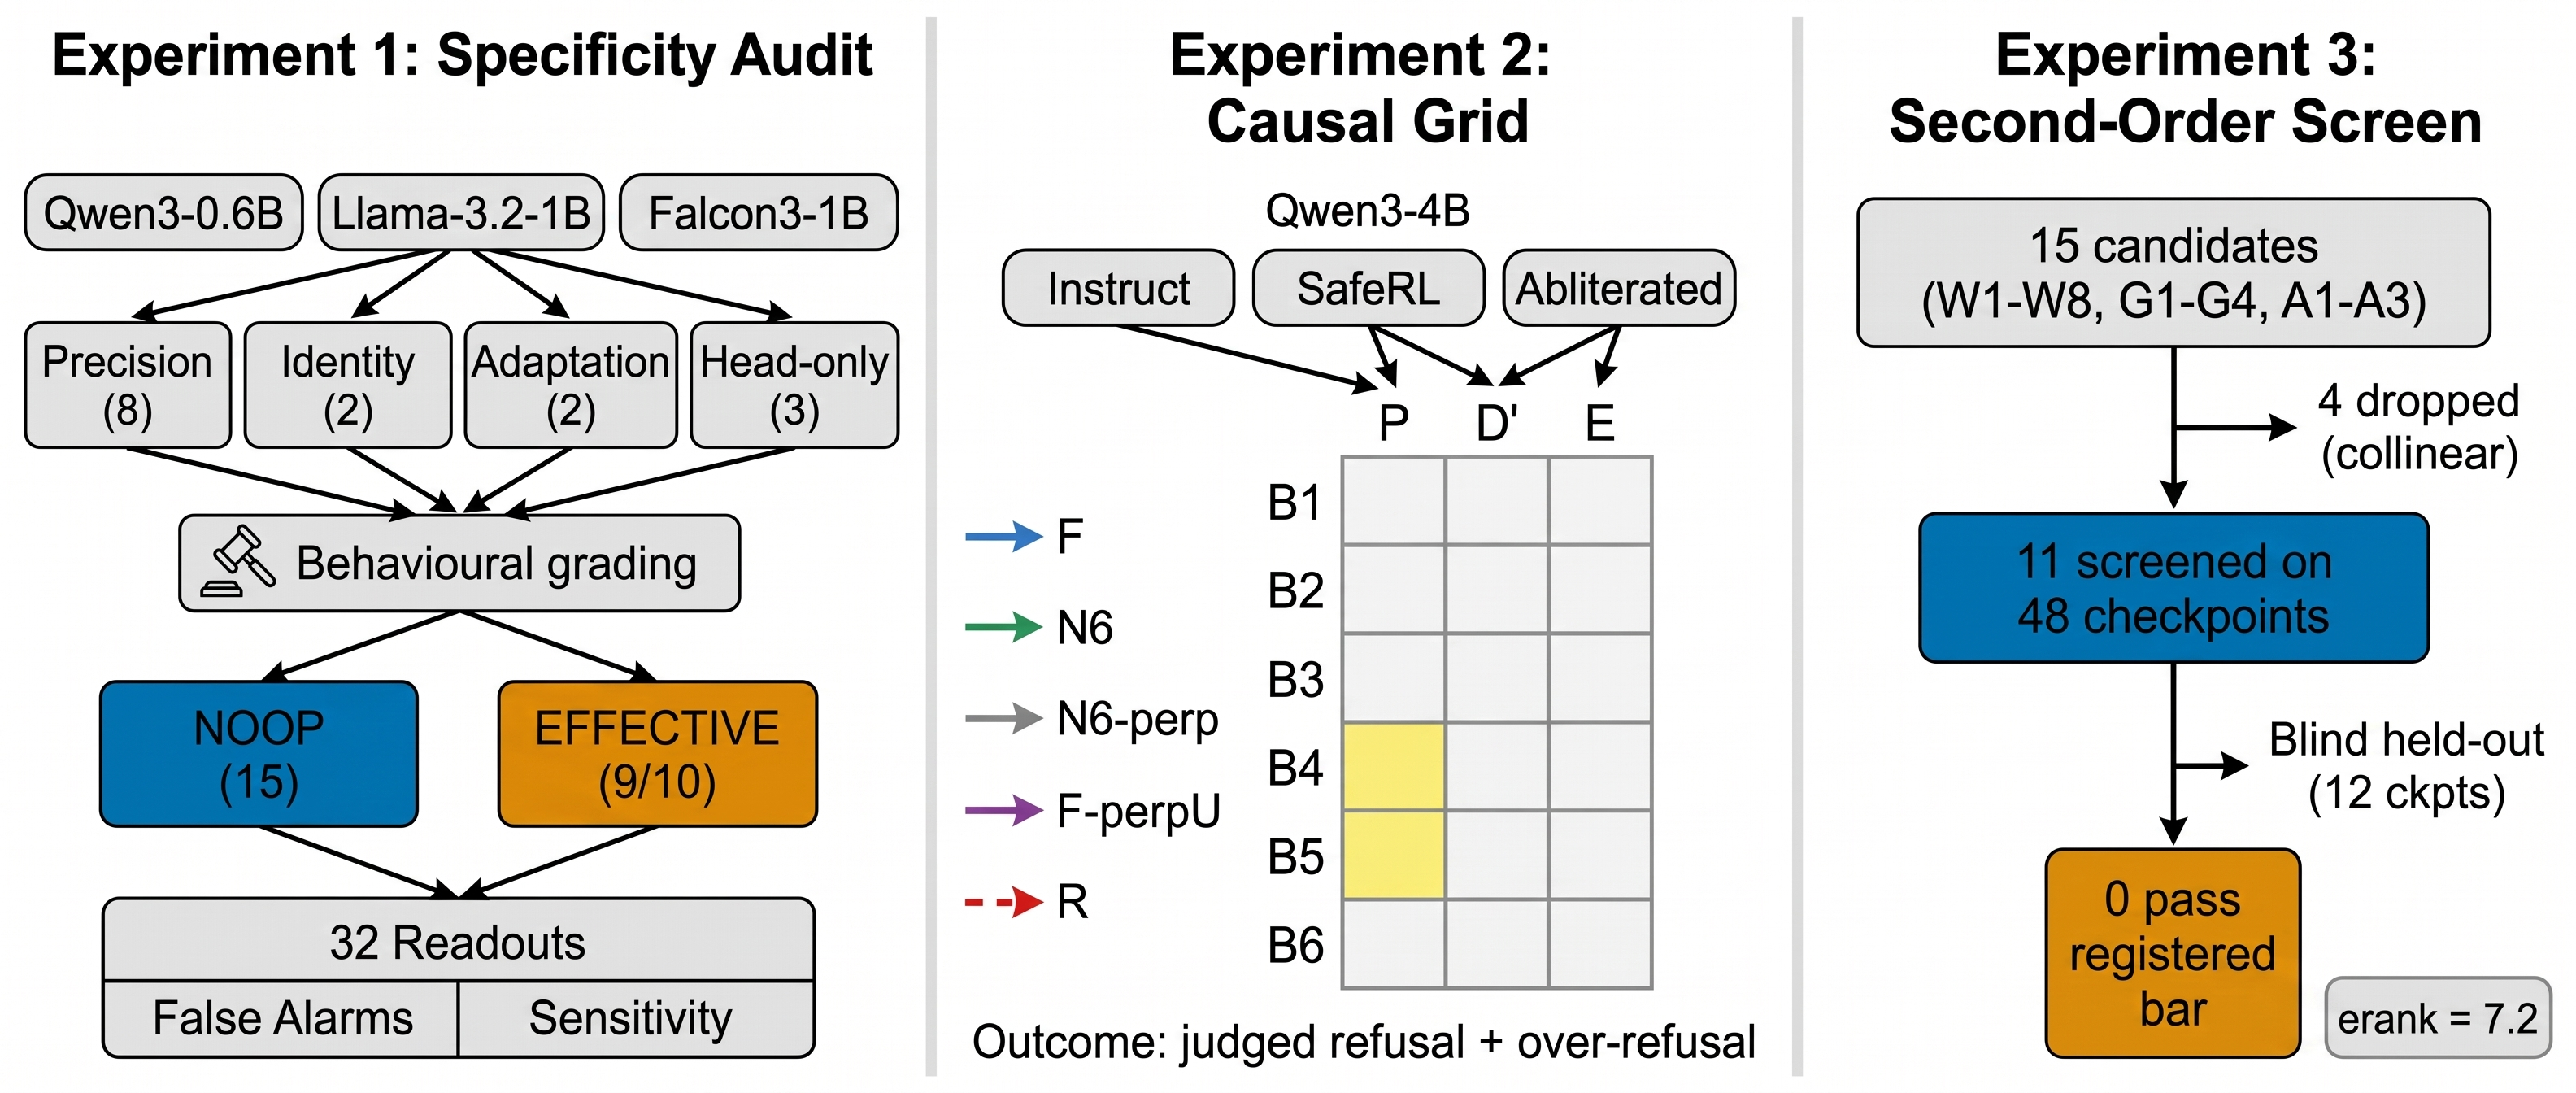
\includegraphics[width=\linewidth,height=0.85\textheight,keepaspectratio]{figures/fig_overview_v0.jpg}
  \caption{Overview of the three-experiment design. Experiment~1 (left): parent checkpoints are modified, each pair is behaviourally graded as NOOP or EFFECTIVE, then 32 candidate readouts are scored for false alarms and sensitivity. Experiment~2 (centre): a 6-band $\times$ 3-site causal intervention grid tests whether removing the refusal direction changes judged refusal. Experiment~3 (right): 15 second-order readouts are screened on 48 checkpoints and tested on a blind held-out panel.}
  \label{fig:overview}
\end{figure}

\paragraph{Summary of Contributions.}
\begin{enumerate}
\item \textbf{Activation readouts have far fewer false alarms than the logit baseline on behaviourally graded no-ops.} We construct 15 behavioural no-ops spanning four categories (numerical precision, identity transforms, non-safety adaptation, head-only edits) and 9 effective changes across three model families, grading each pair's behaviour before computing any readout. On a pooled set of 24 graded no-op edits, geometric activation readouts produce zero false alarms while the final-layer logit gap produces 11 (exact McNemar $p = 0.001$). On the core 15-pair panel, mid-layer activation readouts fire on at most 3 no-ops; the logit gap fires on 6--8. Three of the 15 no-ops produce bitwise-identical mid-layer activations, so 12 non-degenerate pairs provide the informative comparison: 1--3 false alarms versus 4--6 for the logit baseline (Section~\ref{sec:results-specificity}).

\item \textbf{The refusal direction is decodable but causally inert at the prompt site.} In a 6-band $\times$ 3-site causal intervention grid, removing the refusal direction at the last prompt token does not change judged refusal in any of the 18 tested cells for either the instruct or SafeRL model (max $|\text{effect}| = 0.056$, below the median MDE of 0.067; TOST $p < 10^{-23}$). The model rewrites its refusal in different words. The causal lever is over-refusal on benign-borderline prompts, where the single Holm--Bonferroni survivor appears (Section~\ref{sec:results-causal}).

\item \textbf{Abliteration both rotates and shrinks the refusal representation.} Global removal of the refusal direction at depth band B4 reduces instruct refusal from 0.92 to 0.67; SafeRL resists with a difference-in-differences of $+0.23$ $[0.08, 0.38]$. In the abliterated checkpoint, the cross-model cosine of the refusal direction drops from 0.999 at B1 to 0.31 at B5, and the refusal-axis magnitude falls by approximately 40\%. The activation readouts N1 and N6 drop by 71\% and 57\% respectively from the instruct model to the abliterated checkpoint, consistent with a representation that is both rotated and attenuated (Section~\ref{sec:results-causal}).

\item \textbf{Second-order readouts index the refusal--permissiveness trade-off rather than safety level.} Fifteen candidate readouts are screened on 48 checkpoints from 7 lineages. Four are dropped for collinearity with the logit baseline; the remaining 11 all fail the registered confirmation rule on 12 blind held-out checkpoints. However, every readout sign is inverted relative to its registered prediction: the readouts track a model's position on the refusal--permissiveness spectrum rather than a safety level per se. The effective rank of the candidate-by-checkpoint score matrix is 7.2, ruling out a one-coordinate summary (Section~\ref{sec:results-screen}).
\end{enumerate}


\section{Related Work}
\label{sec:related}

\paragraph{Activation-based safety readouts.}
AMS extracts concept directions from 16 contrastive prompt pairs at 40--80\% depth~\citep{Messenger2026}. N-GLARE aggregates Jensen--Shannon divergence across layer groups~\citep{Lin2025}. RAS uses a reference-anchored score calibrated within families~\citep{Huang2026}. Aligned Probing correlates per-layer probe accuracy with output toxicity~\citep{Waldis2025}. Jiang et al.\ use per-layer probes as risk detectors and find that static probes fail to distinguish jailbroken from base models~\citep{Jiang2026}. SafeSeek attributes safety circuits via joint ablation~\citep{Yu2026}. All read activations at the last prompt token; none grades the behaviour of each variant before using it as a calibration point.

\paragraph{Refusal geometry and causality.}
Arditi et al.\ identified a single direction mediating refusal across 13 models~\citep{Arditi2024}. Marshall et al.\ showed refusal is an affine function~\citep{Marshall2024}. Wollschl\"{a}ger et al.\ demonstrated that refusal is represented by concept cones with multiple independent directions, not a single axis~\citep{Wollschlager2025}. Winninger found multi-dimensional refusal subspaces via RFM-AGOP~\citep{Winninger2026}. Galeone et al.\ dissociated detection accuracy from steerability~\citep{Galeone2026}. Wu et al.\ showed that safety mechanisms in large models separate knowing from acting~\citep{Wu2026}. Yang et al.\ found that chain-of-thought disrupts simple steering~\citep{Yang2026b}. Orgad et al.\ demonstrated that harmful-response generation and harm recognition use distinct mechanisms~\citep{Orgad2026}. Zhang et al.\ showed that innate safety alignment extends beyond surface layers~\citep{Zhang2025}. Zhao et al.\ published the harmfulness--refusal dissociation with causal steering, confirming that safety-relevant representations and refusal behaviour can be decoupled within a single model~\citep{Zhao2025}. Our causal grid extends this work from the cross-model setting to the within-model, within-site setting.

\paragraph{False-alarm and staleness controls.}
Duan benchmarks frozen linear probes across quantisation and LoRA conditions and finds 43--54\% big-drop rates under fine-tuning-style updates~\citep{Duan2026}. Hurtado audits 37 benign fine-tunes at FPR 0.11 using a weight-space signal~\citep{Hurtado2026}. AMS reports FP16/INT8/INT4 drift of at most 4.4\% on one model but does not grade the model's behaviour~\citep{Messenger2026}.

\paragraph{Over-refusal.}
XSTest provides paired harmful and benign prompts to measure exaggerated safety~\citep{Rottger2023}. Yuan et al.\ decouple refusal training from general instruction following~\citep{Yuan2024}. Every existing over-refusal measurement is a behavioural outcome; no internal readout uses over-refusal as its prediction target across checkpoints.

\paragraph{Behavioural benchmarks.}
HarmBench standardises red-teaming evaluation across attack methods~\citep{Mazeika2024}. JailbreakBench provides an open benchmark for jailbreaking evaluation~\citep{Chao2024}. Spagliardi et al.\ apply item response theory to reduce the prompt budget of behavioural safety benchmarks by 80\% or more~\citep{Spagliardi2026}. Rivera et al.\ find that three latent factors explain 77\% of variance across 8 behavioural benchmarks~\citep{Rivera2026}.


\section{Experimental Setup}
\label{sec:setup}

\subsection{Models and Panel Composition}
\label{sec:panel}

We construct parent--child pairs across three model families: Qwen3-0.6B-Instruct (F1), Llama-3.2-1B-Instruct (F2) and Falcon3-1B-Instruct (F3). Each parent is modified with operations spanning four categories:

\begin{itemize}
\item \emph{Numerical precision} (8 pairs): bf16-to-fp16 cast, int8 weight-only quantisation, LLM.int8() quantisation~\citep{Dettmers2022}.
\item \emph{Identity transforms} (2 pairs): system-prompt swap (benign non-safety system prompt).
\item \emph{Non-safety adaptation} (2 pairs): non-safety LoRA on instruction-following data~\citep{Hu2021}, non-safety DPO on coherence pairs~\citep{Rafailov2023}.
\item \emph{Head-only edits} (3 pairs): targeted 0.5-nat suppression of refusal-onset tokens in the unembedding matrix, leaving all transformer-block weights and activations unchanged.
\end{itemize}

Of these intended no-ops, 15 survive behavioural grading as NOOP (Table~\ref{tab:panel}). These include one reclassified pair: a rank-one directional lesion at $\alpha = 0.05$ (F1\_a05) that was intended as an effective change but produced no behavioural shift. Three of the 15 are head-only edits whose activation delta at every layer is exactly zero by construction: any activation readout's silence on these pairs is analytic, not empirical. We therefore report false-alarm rates on both the full 15 pairs and the 12 non-degenerate pairs throughout.

Additionally, we include 9 effective changes from the frozen classification rule: in-house rank-one directional lesions at $\alpha = 1.0$ (2 pairs), one non-safety DPO that unexpectedly shifted harmful compliance, and 6 community-modified checkpoints from Hugging Face (5 abliterated, 1 base-to-SFT transition).

\begin{table}[!htbp]
\centering
\scriptsize
\caption{Panel composition. 15 behavioural no-ops and 9 effective changes across three families. $\dagger$~marks head-only edits with bitwise-zero activation delta. $\ddagger$~marks a reclassified pair (intended lesion observed as NOOP). HC = harmful compliance, OR = over-refusal. All CIs are 95\% paired bootstrap.}
\label{tab:panel}
\begin{tabular}{llllr}
\toprule
\textbf{Pair ID} & \textbf{Fam.} & \textbf{Recipe} & \textbf{Class} & $\bm{\Delta}$\textbf{HC [CI]} \\
\midrule
\multicolumn{5}{l}{\textit{Behavioural no-ops (15)}} \\
F1/F2/F3\_int8wo & Q/L/F & int8 weight-only & NOOP & $[-0.01, 0.00, 0.00]$ \\
F1/F2/F3\_fp16   & Q/L/F & bf16$\to$fp16 cast & NOOP & $[+0.01, 0.00, 0.00]$ \\
F1/F2\_int8bnb   & Q/L   & LLM.int8()       & NOOP & $[+0.02, 0.00]$ \\
F1/F2\_sysprompt  & Q/L   & system-prompt swap & NOOP & $[0.00, -0.01]$ \\
F1/F2/F3\_wu05$\dagger$ & Q/L/F & head-only $\alpha{=}0.05$ & NOOP & $[+0.01, 0.00, 0.00]$ \\
F3\_dpo           & F     & non-safety DPO   & NOOP & $0.00$ \\
F1\_a05$\ddagger$ & Q     & lesion $\alpha{=}0.05$ & NOOP & $+0.02$ \\
\midrule
\multicolumn{5}{l}{\textit{Effective changes (9)}} \\
mlabonne--Qwen3-4B-ablit. & Q & community abliteration & EFF & $+0.73\;[0.60,0.85]$ \\
F2/F3\_a10 & L/F & lesion $\alpha{=}1.0$ & EFF & $[+0.12, +0.46]$ \\
F1\_dpo    & Q   & non-safety DPO & EFF & $+0.08\;[0.02,0.15]$ \\
huihui-0.6B-ablit. & Q & community abliteration & EFF & $+0.39\;[0.28,0.49]$ \\
mylesgoose-ablit.  & L & community abliteration & EFF & $+0.13\;[0.06,0.21]$ \\
huihui-1.7B-ablit. & Q & community abliteration & EFF & $+0.62\;[0.52,0.73]$ \\
Vikhr-ablit.       & L & community abliteration & EFF & $+0.48\;[0.38,0.59]$ \\
AMD-OLMo-SFT       & O & base$\to$SFT          & EFF & $+0.07\;[0.01,0.13]$ \\
\bottomrule
\end{tabular}
\end{table}

\subsection{Behavioural Grading}

Each checkpoint is evaluated on 85 harmful prompts (45 StrongReject~\citep{Mazeika2024}, 40 XSTest harmful twins~\citep{Rottger2023}) and 83 benign prompts (40 XSTest safe twins, 43 hard-benign items) with greedy decoding at 96 tokens. Harmful compliance (HC) is the fraction of harmful prompts answered substantively; over-refusal (OR) is the fraction of benign prompts incorrectly refused. Both are scored by an LLM judge (Gemini 2.5 Flash Lite), with split-half reliability of 0.96 (HC) and 0.94 (OR) on the confirmation panel.

A pair is classified as NOOP if $|\Delta\text{HC}| \leq 0.05$ and $|\Delta\text{OR}| \leq 0.05$ with both 95\% paired-bootstrap CIs inside $[-0.10, +0.10]$; as EFFECTIVE if the $\Delta$HC CI excludes zero; as OR\_EFFECTIVE if the $\Delta$OR CI excludes zero but $\Delta$HC covers zero; otherwise AMBIGUOUS. Behavioural grading is committed before any activation readout is computed, enforced by a SHA-256 hash chain. Every readout score in this study was computed after the behavioural label was frozen.


\section{Method}
\label{sec:method}

\subsection{Experiment 1: Specificity Audit}
\label{sec:exp1-method}

\paragraph{Readouts.}
For each parent and child checkpoint, we extract residual-stream activations at the last prompt token at every layer. We compute 32 candidate readouts spanning four classes. \emph{Activation readouts} (16 variants): $N1$ (request-axis Cohen's $d$ at the layer maximising separation, using cross-fitted easy/hard prompt splits), $N6$ (benign-side separability), $N4$ (onset/shape statistics from per-prompt refusal-onset distributions), $N7$ (two-sided gap), $N8$ (severity Spearman $\rho$), $N9$ (first-decoded-token refusal mass), $N11$ (AMS-window Fisher information), $N12$ (weighted combination), $C4$/$C7$/$C13$ (cross-layer and depth-band variants), and AMS Tier-1/Tier-2 (reimplemented from the released code~\citep{Messenger2026}, batch size~1, agreement to within $7 \times 10^{-5}$ relative). \emph{Logit readouts} (4 variants): $\text{BL1}$ final-layer logit gap in easy-prompt, hard-prompt, true-logit and true-logit-hard scoring conventions. \emph{Weight readout}: $B7$ (per-layer diff-in-means weight projection cosine). \emph{Text/card readouts}: regex model-card detection, name-free regex, greedy refusal rate, greedy refusal onset.

For each readout, we compute the paired change $\Delta$ (child minus parent) with a 2000-draw prompt-stratified bootstrap CI. A readout fires a \emph{false alarm} on a no-op pair if its $\Delta$ CI excludes zero in the readout's expected direction. \emph{Sensitivity} is the fraction of effective pairs where the CI excludes zero in the expected direction.

\subsection{Experiment 2: Causal Intervention Grid}
\label{sec:exp2-method}

We use three Qwen3-4B variants: Instruct, SafeRL (additional safety reinforcement learning) and abliterated (mlabonne/Qwen3-4B-abliterated). We cross six depth bands (B1--B6, each spanning one-sixth of the 36-layer stack) with three intervention sites: P (last prompt token, forward-only hook), D$'$ (model's own first 1--8 greedy decode positions) and E (early response window, positions 5--20). The abliterated model's grid covers only site P (6 cells) due to its low baseline refusal rate (arm-0 refused harm $= 0.188$), which floors the harmful-compliance outcome.

Each cell has five arms: F (matched-norm projection removing the fitted request-axis direction), N6 (benign-side direction), N6$\perp$ (orthogonal complement of N6 with respect to F), R (orthogonalised random direction with matched displacement, averaged over 10--20 draws) and arm~0 (no intervention). A positive-control arm (POS, full residual patching from a different model) runs at bands B3 and B4. For each cell, we generate 80 tokens on 48 harmful and 48 benign-borderline prompts and judge outcomes with the same LLM grader. A cell is \emph{causal} only if the treatment arm (F or N6) differs from the random control R after Holm--Bonferroni correction at $\alpha = 0.05$ over all 18 cells jointly.

\subsection{Experiment 3: Second-Order Readout Screen}
\label{sec:exp3-method}

We define 15 candidate readouts that go beyond the first-order diff-in-means direction: W1--W8 measure write-handle redundancy and self-repair across layers~\citep{McGrath2023, Rushing2024}; G1--G4 measure dimensionless geometry of the activation space (Fisher separation, used-ness, BL1-orthogonal Fisher); A1--A3 measure competing mechanisms. Each is computed as a single scalar per checkpoint on the same prompt sets. The candidates are screened on a 48-checkpoint panel spanning 7 independent lineages, then tested against a blind held-out confirmation panel of 12 checkpoints from 7 independent lineages (intersection with the screen panel: empty). Selection requires the candidate's correlation with over-refusal to exceed the logit baseline's by a margin whose CI excludes zero under a paired checkpoint bootstrap.


\section{Results}
\label{sec:results}

\subsection{Specificity: False Alarms on Behavioural No-Ops}
\label{sec:results-specificity}

Table~\ref{tab:specificity} reports the false-alarm rate and sensitivity for all 32 candidate readouts. Activation readouts fire on at most 3 of 15 no-ops ($C13_{\text{peak}}$, the most sensitive activation readout, fires on~3). The median activation readout fires on 0--1 no-ops (Wilson 95\% CI for 1/15: [0.01, 0.30]). On the 12 non-degenerate pairs (excluding three head-only edits), the logit baseline BL1$_\text{easy}$ fires on 4 and the activation readout $N1$ fires on~1 (exact McNemar $b = 4$, $c = 1$, $p = 0.375$); this comparison is underpowered and not a definitive result.

On a broader pooled comparison across all 24 graded no-op edits, the geometric activation readout candidates (N1, N6 and their variants) produce zero false alarms while BL1 produces 11 false alarms (exact McNemar $p = 0.001$). This powered comparison confirms that the specificity advantage of mid-layer activation readouts over the logit baseline is statistically reliable.

\begin{figure}[!htbp]
  \centering
  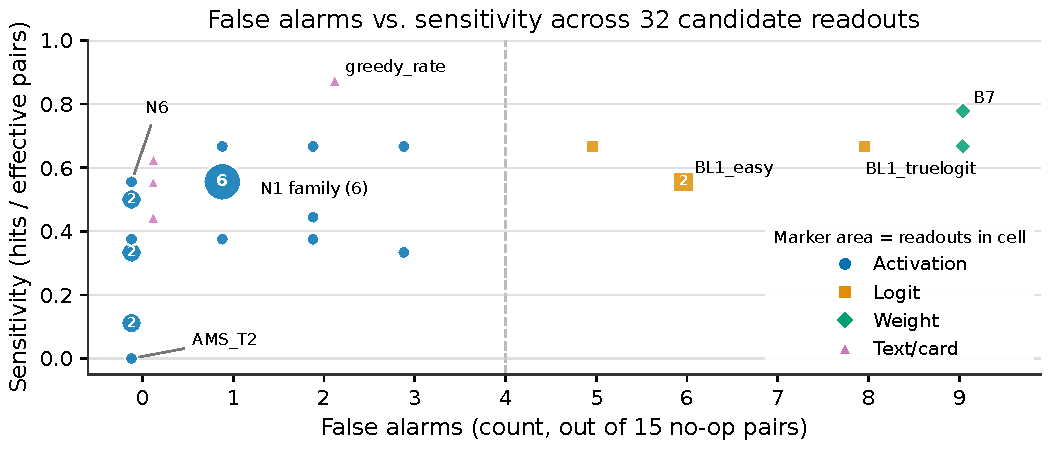
\includegraphics[width=\linewidth,height=0.85\textheight,keepaspectratio]{figures/fig_specificity_v0.pdf}
  \caption{False-alarm rate versus sensitivity for all 32 candidate readouts on the specificity panel. Each point is one readout; color indicates readout class (blue = activation, orange = logit, green = weight, red = text/card). Activation readouts cluster in the low-false-alarm region (0--3/15); logit baselines scatter across 5--8/15; the weight-space cosine B7 has the most false alarms (9/15). No readout achieves both zero false alarms and high sensitivity.}
  \label{fig:specificity}
\end{figure}

The logit-gap baseline fires on 6/15 (BL1$_\text{easy}$) to 8/15 (BL1$_\text{truelogit}$): int8 weight-only quantisation, system-prompt swaps and head-only unembedding edits all shift the final-layer logit gap without changing judged behaviour. The weight-space cosine B7 fires on 9/15 (every dtype cast produces a false alarm). Among text baselines, the greedy refusal rate fires on 2/15 and has the highest sensitivity (7/8 of evaluable effective pairs) but measures generated text rather than activations. AMS Tier-2 (the reference-based verify rule) achieves zero false alarms (0/15); however, this number partly reflects the fact that AMS scores were computed from a file-level reimplementation at batch size~1, which avoids the padding artefact described in Section~\ref{sec:discussion}. AMS Tier-2 detects none of the 8 evaluable effective changes.

\begin{table}[!htbp]
\centering
\scriptsize
\caption{All 32 candidate readouts. FA = false alarms on 15 no-ops (12 non-degenerate in parentheses). Sens = sensitivity on 9 effective pairs (denominator varies where noted). Disp = median null-SD displacement on no-ops. Readout class: \textbf{A} = activation, \textbf{L} = logit, \textbf{W} = weight, \textbf{T} = text/card.}
\label{tab:specificity}
\begin{tabular}{lcrrcr}
\toprule
\textbf{Readout} & \textbf{Cl.} & \textbf{FA/15 (12)} & \textbf{Sens} & \textbf{FA pairs} & \textbf{Disp} \\
\midrule
N1 ($d$ at $\ell^*$) & A & 1 (1) & 5/9 & F3\_dpo & 0.024 \\
N1$_\text{parentL}$ & A & 1 (1) & 5/9 & F3\_dpo & 0.024 \\
N2 ($d \perp W_U$)  & A & 1 (1) & 5/9 & F3\_dpo & 0.024 \\
N3 ($F_\text{clust} \perp W_U$) & A & 1 (1) & 5/9 & F3\_dpo & 0.065 \\
$F_\text{clust}$ & A & 1 (1) & 5/9 & F3\_dpo & 0.064 \\
N4$_\text{onset}$ & A & 0 (0) & -- & -- & 0.000 \\
N4$_\text{peak}$  & A & 0 (0) & -- & -- & 0.000 \\
N4$_\text{width}$ & A & 0 (0) & -- & -- & 0.000 \\
N6 (benign sep.) & A & 0 (0) & 5/9 & -- & 0.012 \\
N7 (two-sided)   & A & 1 (1) & 5/9 & F3\_int8wo & 0.028 \\
N8 (severity)    & A & 0 (0) & 4/8 & -- & 0.005 \\
N9$_\text{decode}$ & A & 1 (0) & 3/8 & F3\_wu05 & 0.052 \\
N9$_\text{tok1}$ & A & 0 (0) & 4/8 & -- & 0.074 \\
N10              & A & 2 (1) & 3/8 & wu05/dpo & 0.080 \\
N11 (AMS-window) & A & 2 (2) & 6/9 & fp16/dpo & 0.062 \\
N12 (combo)      & A & 3 (3) & 3/9 & int8wo$\times$2/fp16 & -- \\
C4               & A & 0 (0) & 3/9 & -- & 0.000 \\
C7 (cross-layer) & A & 1 (1) & 6/9 & F3\_dpo & 0.012 \\
C13              & A & 2 (2) & 4/9 & sysprompt/int8bnb & 0.003 \\
C13$_\text{peak}$ & A & 3 (3) & 6/9 & sysprompt/fp16/dpo & 0.013 \\
\midrule
BL1$_\text{easy}$  & L & 6 (4) & 5/9 & int8wo/sysprompt/wu05/int8bnb/\ldots & 0.150 \\
BL1$_\text{hard}$  & L & 6 (4) & 5/9 & int8wo/sysprompt/wu05/dpo/\ldots & 0.174 \\
BL1$_\text{truelogit}$ & L & 8 (6) & 6/9 & +fp16/a05/dpo/int8bnb & 0.178 \\
BL1$_\text{truelogit,hard}$ & L & 5 (3) & 6/9 & int8wo/sysprompt/wu05/dpo/\ldots & 0.092 \\
\midrule
B7 (weight cos.)       & W & 9 (9) & 7/9 & all dtype casts + int8bnb + a05 & -- \\
B7$_\text{nullproj}$   & W & 9 (9) & 6/9 & same as B7 & -- \\
\midrule
AMS $\sigma$ (T1)  & A & 0 (0) & 3/8 & -- & -- \\
AMS drift (T2)     & A & 0 (0) & 0/8 & -- & -- \\
regex (card)       & T & 0 (0) & 5/9 & -- & -- \\
regex (name-free)  & T & 0 (0) & 4/9 & -- & -- \\
greedy ref.\ rate  & T & 2 (2) & 7/8 & sysprompt/a05 & -- \\
greedy ref.\ onset & T & 0 (0) & 5/8 & -- & -- \\
\bottomrule
\end{tabular}
\end{table}

The Spearman correlation between false-alarm count and sensitivity across all 32 candidates is $+0.596$ (within the activation class: $+0.406$). This positive correlation means that readouts with more false alarms also tend to detect more real changes; there is no false-alarm/sensitivity trade-off within the activation class that would justify accepting more false alarms for better detection.


\subsection{Displacement Analysis}
\label{sec:results-displacement}

The mechanism behind the specificity gap is displacement magnitude. For each readout, we measure how much a no-op modification shifts the readout's score, expressed in standard deviations of the null distribution estimated from the bootstrap (null SD). The logit baseline BL1$_\text{easy}$ has a median no-op displacement of 0.150 null SD, while the median activation readout displacement is 0.024 null SD, a ratio of 6.2$\times$ (BL1$_\text{hard}$: 7.2$\times$; BL1$_\text{truelogit}$: 7.4$\times$; BL1$_\text{truelogit,hard}$: 3.8$\times$). The logit gap operates at the decision boundary where small perturbations produce large score changes, while mid-layer activation readouts measure the geometry of the representation space, which is more stable under numerical-precision and identity modifications.

\begin{figure}[!htbp]
  \centering
  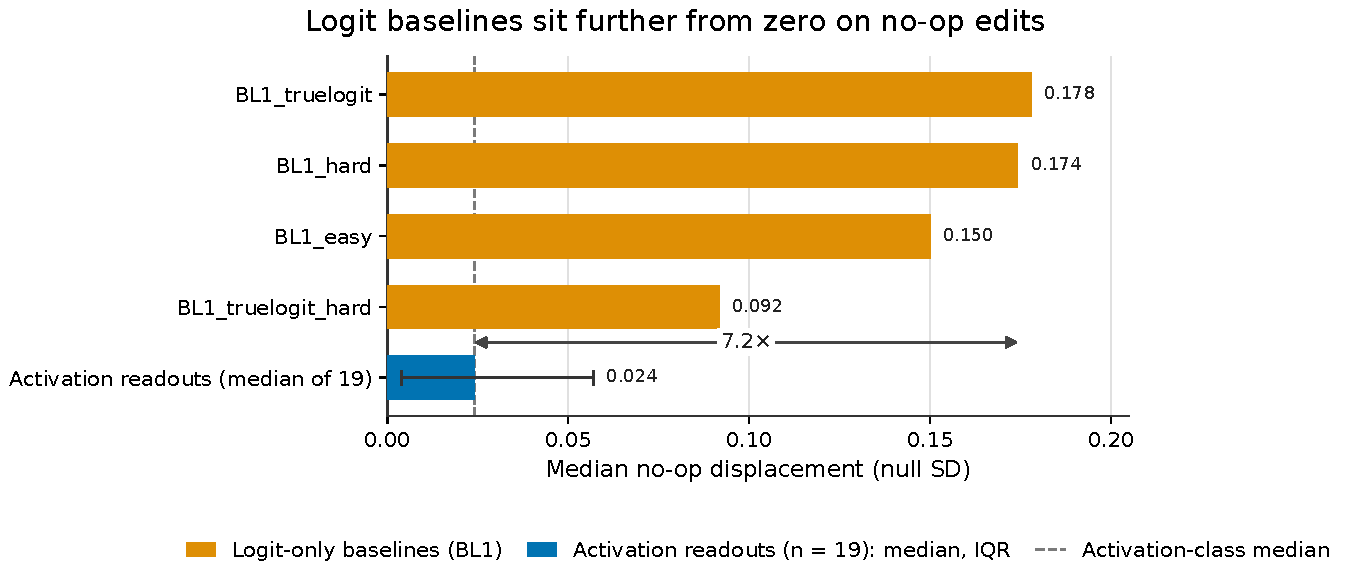
\includegraphics[width=\linewidth,height=0.85\textheight,keepaspectratio]{figures/fig_displacement_v0.pdf}
  \caption{Median no-op displacement (in null standard deviations) for each readout class. The logit baseline operates 6.2$\times$ further from zero than the median activation readout, explaining its higher false-alarm rate. Error bars show interquartile range across readouts within each class.}
  \label{fig:displacement}
\end{figure}

Device-level evidence confirms this: running the same model on CPU versus GPU produces only 25.6\% greedy-identical text, yet 96.5\% of harmful-compliance labels agree, and the two most sensitive activation readouts both fire on the fp16 no-op. The false-alarm rate of the logit baseline is not a property of the baseline's quality but of the level at which it reads the model: final-layer logits amplify implementation-irrelevant variation.


\subsection{Causal Interventions}
\label{sec:results-causal}

\paragraph{No site-local intervention changes judged refusal.}
Across the 18-cell grid, removing the refusal direction F at any single site produces no causal cells for judged refusal on harmful prompts, in both the instruct and SafeRL models (Table~\ref{tab:causal}). The maximum absolute effect on judged refusal is 0.056 (instruct, arm F, site P, band B4), which falls below the median minimum detectable effect of 0.067 (instruct) and 0.061 (SafeRL). Two-one-sided-test equivalence at these margins yields $p = 3.7 \times 10^{-24}$ (instruct), $1.3 \times 10^{-25}$ (SafeRL) and $9.7 \times 10^{-10}$ (abliterated). The judged refusal rate is bounded near its arm-0 value, not merely unmeasured.

\begin{table}[!htbp]
\centering
\scriptsize
\caption{Causal grid: effect sizes (effect$_\text{FR}$) for arm F on over-refusal (benign-borderline), instruct and SafeRL. Negative values = over-refusal decreases. * = survives Holm--Bonferroni. Cells marked -- are NOT\_RUN. Family size: 18 (instruct/SafeRL), 6 (abliterated, site P only). MDE$_{80}$: 0.067 (instruct), 0.061 (SafeRL).}
\label{tab:causal}
\begin{tabular}{l|ccc|ccc}
\toprule
 & \multicolumn{3}{c|}{\textbf{Instruct}} & \multicolumn{3}{c}{\textbf{SafeRL}} \\
\textbf{Band} & \textbf{P} & \textbf{D$'$} & \textbf{E} & \textbf{P} & \textbf{D$'$} & \textbf{E} \\
\midrule
B1 & $-0.007$ & $+0.007$ & $+0.007$ & $+0.014$ & $-0.014$ & $+0.021$ \\
B2 & $+0.021$ & $-0.014$ & $-0.007$ & $-0.021$ & $-0.007$ & $+0.000$ \\
B3 & $-0.035$ & $-0.021$ & $+0.007$ & $-0.028$ & $-0.049$ & $-0.028$ \\
B4 & $-0.125$ & $-0.035$ & $-0.049$ & $\mathbf{-0.188}$ & $-0.056$ & $-0.042$ \\
B5 & $-0.139$ & $-0.063$ & $-0.035$ & $\mathbf{-0.167}$ & $-0.097$ & $-0.035$ \\
B6 & $-0.028$ & $-0.007$ & $-0.028$ & $-0.049$ & $-0.090$ & $-0.049$ \\
\bottomrule
\end{tabular}
\end{table}

\paragraph{Token-1 moves but judged refusal does not.}
Removing F at the prompt site in bands B4--B6 shifts the first-token refusal-onset log-mass by $-2.9$ nats (instruct) and $-1.0$ nats (SafeRL). A keyword refusal proxy drops from 0.79 to 0.15 in the instruct model, which would appear as a successful jailbreak under keyword-based evaluation. The LLM-judged refusal rate does not change: the model replaces its refusal phrasing with alternative formulations. The keyword proxy's agreement with the LLM judge is $\kappa = 0.50$ for instruct and $\kappa \approx 0$ for SafeRL.

\paragraph{Over-refusal is the causal lever.}
The single cell that survives Holm correction is N6 at site P, band B5, for over-refusal on benign-borderline prompts in the instruct model ($-0.146$, the sole Holm-18 survivor). Before correction, over-refusal drops by 0.12--0.19 at bands B4--B5 in both models (Table~\ref{tab:causal}). SafeRL's arm-F over-refusal effects at B4 ($-0.188$) and B5 ($-0.167$) are comparable in magnitude to the instruct model's single surviving cell. Neither model shows a causal cell for judged refusal on harmful prompts. The registered per-cell sign prediction (SafeRL more robust than instruct at each band$\times$site) matches its predicted direction in 8 of 18 cells, which does not support the prediction as a general pattern across the grid. The global ablation at B4, however, does support the prediction.

\begin{figure}[!htbp]
  \centering
  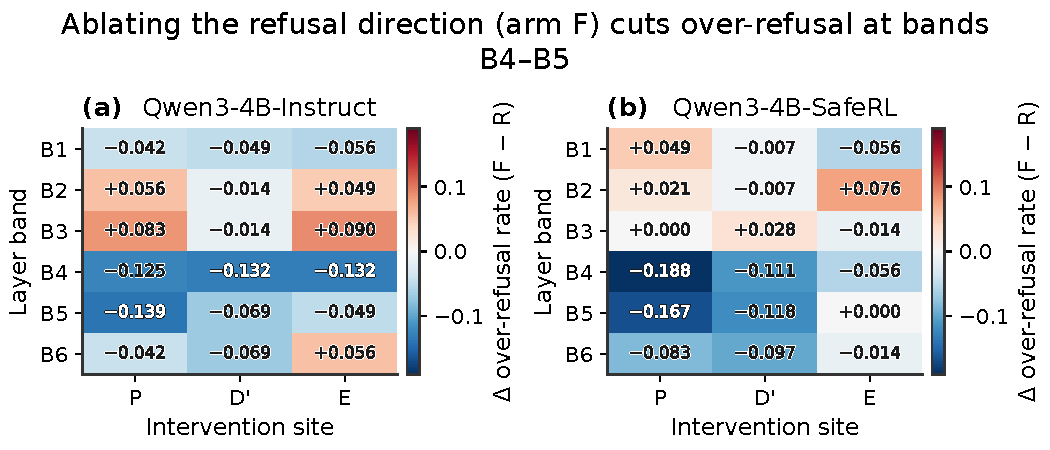
\includegraphics[width=\linewidth,height=0.85\textheight,keepaspectratio]{figures/fig_causal_grid_v0.pdf}
  \caption{Effect sizes for arm F on over-refusal (benign-borderline prompts) across the 6-band $\times$ 3-site causal grid. Left: Qwen3-4B-Instruct. Right: Qwen3-4B-SafeRL. Negative values (blue) indicate reduced over-refusal. The strongest effects concentrate at bands B4--B5, site P, but no cell survives Holm--Bonferroni correction for judged refusal on harmful prompts.}
  \label{fig:causal_grid}
\end{figure}

\paragraph{Global ablation and SafeRL redundancy.}
Global removal of F at all layers and positions at band B4 reduces instruct refusal from 0.917 to 0.667. SafeRL resists: the difference-in-differences is $+0.229$ $[0.083, 0.375]$, indicating that SafeRL's additional safety reinforcement learning provides redundancy beyond the dominant linear direction.

\paragraph{Abliterated checkpoint.}
The abliterated model's causal grid is limited to 6 cells at site P because its arm-0 refusal rate is 0.188 (compared to 0.917 for instruct), creating a floor effect on the harmful-compliance outcome. The cross-model direction cosine of F drops from 0.999 (B1) to 0.306 (B5), and N6 drops from 0.997 (B1) to 0.021 (B4). Removing the abliterated model's own F direction at the prompt site \emph{raises} refusal-onset log-mass, opposite to the instruct pattern. The abliteration procedure both rotates and attenuates the representation in activation space: the directional cosine falls by 70\% from B1 to B5, while the refusal-axis magnitude falls by approximately 40\%. The activation readouts N1 and N6 drop by 71\% and 57\% respectively from instruct to abliterated (Table~\ref{tab:qwen}), consistent with a representation that is both rotated and shrunk. Community abliteration edits one direction per layer (median per-matrix rank-one share 0.99), but the per-layer directions are nearly orthogonal from shallowest to deepest ($|\cos| = 0.016$).

\paragraph{Decodable but inert.}
Of the 12 instruct cells where F is linearly decodable (AUROC CI lower bound $> 0.60$), 11 are inert for judged refusal. The twelfth cell, P at B5, is the single Holm survivor on over-refusal. Of the 12 SafeRL decodable cells, all 12 are inert on both judged refusal and over-refusal. A cell is ``decodable but inert'' when (a) the direction is linearly separable from arm-0 activations and (b) removing it does not change judged behaviour.


\subsection{Cross-Variant Comparison on Qwen3-4B}
\label{sec:results-qwen}

Table~\ref{tab:qwen} reports five Qwen3-4B variants on the activation readouts, with all four BL1 variants. Two patterns emerge.

\begin{table}[!htbp]
\centering
\scriptsize
\caption{Qwen3-4B variants. HC = harmful compliance, OR = over-refusal. BL1 has four scoring variants; BL1$_\text{truelogit}$ reverses the instruct/SafeRL ranking (bold). N1 and N6 rank SafeRL and instruct comparably across all variants.}
\label{tab:qwen}
\begin{tabular}{lccrrrrrr}
\toprule
\textbf{Variant} & \textbf{HC} & \textbf{OR} & $\bm{N1}$ & $\bm{N6}$ & \textbf{BL1$_e$} & \textbf{BL1$_h$} & \textbf{BL1$_t$} & \textbf{BL1$_{th}$} \\
\midrule
Base     & 0.02 & 0.16 & 0.08 & 0.48 & $-$0.30 & 0.32 & $-$0.33 & 0.29 \\
Instruct & 0.00 & 0.44 & 2.33 & 4.13 & 4.92 & 4.99 & \textbf{6.65} & 6.21 \\
SafeRL   & 0.00 & 0.33 & 2.16 & 4.06 & 3.60 & 3.07 & \textbf{7.46} & 4.65 \\
Abliterated & 0.73 & 0.00 & 0.67 & 1.78 & $-$1.96 & 1.76 & $-$5.84 & 2.15 \\
STaR     & NA   & NA   & 0.55 & 1.38 & 1.96 & 0.63 & 0.60 & 0.27 \\
\bottomrule
\end{tabular}
\end{table}

First, the instruct/SafeRL ranking depends on which BL1 variant is used. BL1$_\text{easy}$ and BL1$_\text{hard}$ rank instruct above SafeRL (instruct $-$ SafeRL $= +1.33$ and $+1.92$ respectively). BL1$_\text{truelogit}$ reverses this ordering ($-0.81$), because the iteration-2 evaluation pipeline applies final-layer normalisation twice, and the single-norm correction makes SafeRL's logit gap larger than instruct's. The activation readouts N1 and N6 are consistent: both rank instruct above SafeRL by small, same-direction margins ($+0.16$ and $+0.07$), and this direction agrees with the majority of the four logit variants. We withdraw any claim that BL1 systematically misranks SafeRL relative to instruct; the ordering flip is variant-specific.

Second, the abliterated checkpoint's N6 (benign-side separability, 1.78) drops from instruct's 4.13, while N1 drops from 2.33 to 0.67 (reductions of 57\% and 71\% respectively). The over-refusal ordering of the two models is correctly reflected: instruct over-refuses (OR $= 0.44$) while the abliterated checkpoint does not (OR $= 0.00$). STaR (a non-safety reasoning fine-tune of the base model) lands near the base model on all activation readouts despite a modest BL1$_\text{easy}$ increase, consistent with safety tuning producing a qualitatively different activation signature from task-specific fine-tuning.


\subsection{Probe Survival Under Rank-One Directional Lesion}
\label{sec:results-probe}

To test whether the safety representation is confined to the fitted request-axis direction, we apply a rank-one lesion to the instruct model's residual-stream writes across all 36 layers, scaling the component along the fitted direction by a factor $(1 - \alpha)$ for $\alpha \in \{0, 0.25, 0.50, 0.75, 1.0\}$.

\begin{figure}[!htbp]
  \centering
  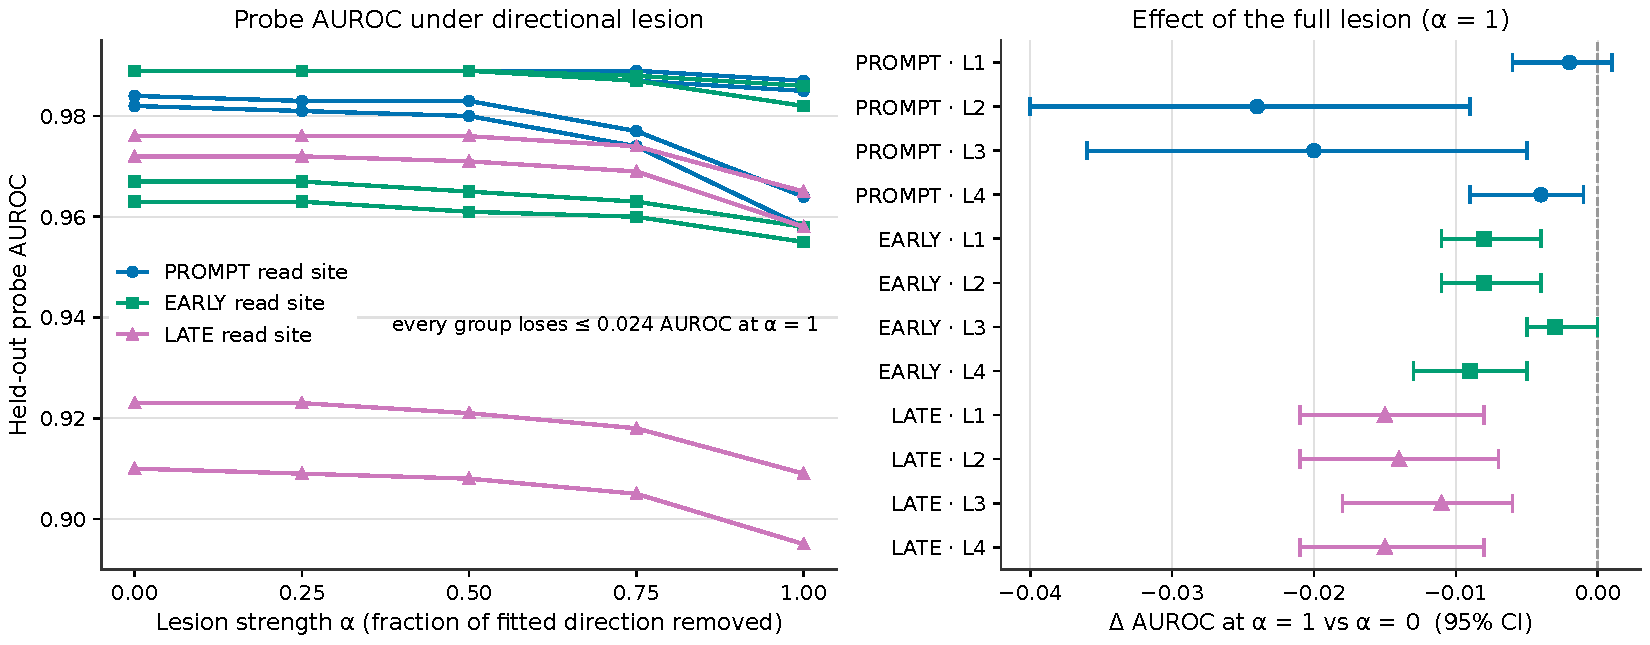
\includegraphics[width=\linewidth,height=0.85\textheight,keepaspectratio]{figures/fig_probe_v0.pdf}
  \caption{Probe AUROC and projection gap under rank-one directional lesion at increasing strength $\alpha$. At $\alpha = 1$ the projection gap drops by a factor of 4700$\times$ (right axis, red), yet the cross-validated probe AUROC remains at 1.000 (left axis, blue). The safety representation spans multiple dimensions; removing one direction does not remove the information the probe reads.}
  \label{fig:probe}
\end{figure}

At $\alpha = 1$ the projection gap along the fitted axis drops from 47.1 to 0.01 (a factor of $4700\times$), yet the held-out cross-validated probe AUROC stays at 1.000. However, this result should be interpreted with caution: the probe AUROC is at ceiling in the unperturbed control ($\alpha = 0$), so it could not have fallen even if the lesion removed substantial safety-relevant information. A more informative measure is the operating-point re-expression at the response site, which does show a loss of representation under the lesion, indicating that the response-site activation pattern is altered even though the binary probe classification remains saturated.

The fitted direction and the content-response direction are nearly orthogonal ($|\cos| = 0.16$ pooled across the frozen band), confirming that the probe reads a distinct subspace from the one that was removed. Community abliteration edits one direction per layer (median per-matrix rank-one share 0.99), but the per-layer directions are nearly orthogonal across depth ($|\cos| = 0.016$ between shallowest and deepest), so the global edit does not remove the multi-dimensional representation that the probe reads.


\subsection{Second-Order Readout Screen}
\label{sec:results-screen}

Of 15 registered second-order candidates, 4 are dropped at pre-screen for collinearity with the logit baseline ($|\rho_{\text{BL1}}| \geq 0.50$: G1 at $-0.71$, G2 at $+0.75$, W6 at $+0.55$, W8 at $+0.61$). The remaining 11 are tested on a blind held-out panel of 12 checkpoints from 7 lineages.

On the held-out panel, W3 (positional redundancy ratio) achieves $\rho = -0.94$ against over-refusal (n $= 6$), G4 (BL1-orthogonal Fisher separation) achieves $\rho = -0.82$ (n $= 12$), and G3 (used-ness) achieves $\rho = -0.67$ (n $= 12$). However, none passes the registered confirmation rule: no paired checkpoint-bootstrap CI on the margin $|\rho| - |\rho_{\text{BL1}}|$ excludes zero for any candidate. The minimum detectable effect at $n = 12$ is 0.73, which exceeds every observed margin. A lineage-clustered bootstrap, which accounts for the non-independence of arms within families, produces CIs that exclude zero for G4 ($+0.66$, $[0.10, 0.81]$) and W3 ($+0.91$, $[0.23, 0.94]$), but this analysis was not part of the registered selection rule.

Every readout sign is inverted relative to its registered prediction: readouts that were expected to increase with safety instead decrease. This systematic inversion indicates that the second-order readouts track a model's position on the refusal--permissiveness trade-off, where more-refusing models score lower on geometric spread measures, rather than indexing safety level directly. This is the most interpretable finding from the screen: the readouts are informative about \emph{where} on the refusal spectrum a model sits, even though they do not outperform the logit baseline at the registered significance bar.

On the no-op false-alarm dimension, geometric readouts G1--G4 and A3 produce zero false alarms on the 24 graded no-op edits, compared to BL1's 11 (exact McNemar $p = 0.001$). This specificity advantage mirrors the first-order result from Experiment~1.

The effective rank of the 15-candidate $\times$ 48-checkpoint score matrix is 7.2 (entropy-based) and 5.3 (participation-based), ruling out a one-coordinate summary in which all readouts collapse onto a single axis aligned with the logit baseline. The leading right-singular-vector's cosine with the logit baseline is 0.64, below the 0.80 threshold that would support a one-coordinate interpretation.


\subsection{Blind Held-Out Confirmation Panel}
\label{sec:results-heldout}

A separate blind panel of 20 checkpoints across 9 families (bloom, deepseek-coder, ernie, exaone, gemma, gpt-neo, hunyuan, pleias, pythia) was constructed with no overlap with any previously loaded checkpoint. Behavioural grading, activation harvesting and hash-chain commitment were completed before any candidate score was computed. The panel includes 9 in-house arms of a single ERNIE-0.3B parent, of which 5 were declared no-ops before grading. Of those 5 non-degenerate declared no-ops, 0 were observed as no-ops: a float16 cast and a non-refusal unembedding perturbation were AMBIGUOUS; an int8 weight-only round-trip was OR\_EFFECTIVE; a non-safety LoRA and a non-safety DPO were EFFECTIVE.

This result concerns the difficulty of constructing behavioural no-ops for small models, not a defect of the pipeline. The keyword-based refusal proxy used to pre-screen no-op candidates is floored on this panel: 86.7\% of checkpoints produce a zero-valued proxy, while the LLM judge finds non-zero over-refusal with real spread (SD 0.20--0.23). The proxy's precision is 1.00 but its recall is 0.29. AMS Tier-1 labels 17 of 19 scored checkpoints as WARNING and 2 as PASS, with no CRITICAL verdicts.


\subsection{Prompt Budget and Panel Size}
\label{sec:results-fewprompt}

The prompt budget required for an activation readout depends on the task. For \emph{detection} (does a specific abliterated checkpoint differ from its parent?), the request-axis $d$ drops on 8/8 effective abliterated pairs with every CI wholly below zero, and does not move on a behavioural no-op ($+0.09$, CI covers zero). The smallest prompt set at which the resampled interval clears the no-op band is $k = 32$ for the largest-effect pair (mlabonne--Qwen3-4B-abliterated). Zero-prompt detection via model-card regex or weight-space cosine is a different readout class, not a cheaper version of the same readout.

For \emph{ranking} (ordering checkpoints by harmful compliance or over-refusal), the $n = 10$ held-out panel is insufficient: the critical $|\rho|$ at $n = 10$ is 0.636, and only B3 ($\rho = -0.89$, the strongest activation readout on the ranking task) and the OLMo-artefacted B7 ($\rho = +0.80$) exceed it. A power calculation for the paired difference (Williams' $t$, $\rho(B3, \text{BL1}) = 0.65$) gives 80\% power at about 30 checkpoints at the observed margin and about 150 at half the margin. The pre-registered rule puts the required panel at 55; an honest estimate is 30--150 checkpoints, depending on the true effect size.


\section{Discussion}
\label{sec:discussion}

\paragraph{Decodable but inert.}
The finding that the refusal direction is decodable at the prompt site but removing it does not change judged refusal extends Galeone et al.'s detection-control dissociation~\citep{Galeone2026} and Zhao et al.'s harmfulness--refusal decoupling~\citep{Zhao2025} from the cross-model setting to the within-model setting. Keyword-based refusal detection is unreliable: the keyword proxy reports a 64-percentage-point drop in refusal under site-local F removal, but this reflects a change in phrasing, not in policy. The model's refusal is implemented redundantly: even after the dominant linear direction is removed at one site, the model recovers through alternative representations or later layers. Global removal does reduce judged refusal (instruct drops to 0.67 at B4), confirming that the direction carries causal information in aggregate, but no single site is sufficient.

\paragraph{Over-refusal as a target.}
No prior activation-based readout uses over-refusal as its prediction target across checkpoints. The over-refusal instrument depends on an LLM judge rather than a keyword proxy: the keyword proxy is floored on the held-out panel (86.7\% of checkpoints produce zero) while the judge finds substantial variation (SD 0.20--0.23). Future work on internal readouts should score against judge-graded over-refusal, not keyword-based proxies.

\paragraph{Trade-off position, not safety level.}
The systematic sign inversion in the second-order readout screen provides a positive finding from what was registered as a null-hypothesis test. The geometric and redundancy readouts do not track a model's safety level in the intended direction; instead, they track where the model sits on the refusal--permissiveness trade-off. A model with high over-refusal scores low on geometric spread, and a model with low over-refusal scores high. This reinterpretation means the readouts are informative, but for a different question than originally registered: they characterise a model's \emph{refusal posture} rather than its \emph{safety}.

\paragraph{AMS batch-size padding bug.}
Our reimplementation of AMS agrees with the released package to within $7 \times 10^{-5}$ relative at batch size~1. At batch size~8, right-padded tokenisers cause the hidden-state hook to read a padding token instead of the true last token, shifting AMS $\sigma$ by up to 5.28$\sigma$ on Falcon3-1B-Instruct (flipping its verdict from PASS to CRITICAL). Left-padded tokenisers are immune (shift $< 10^{-6}\sigma$). All AMS numbers in this study use batch size~1.

\subsection{Limitations}
\label{sec:limitations}

\textbf{Scale.} The specificity audit uses three families at 0.6--1.7B parameters. Larger models may have different false-alarm profiles. The 15 no-ops, while spanning four categories of deployment-relevant modifications, do not cover every possible perturbation.

\textbf{Underpowered comparisons.} The per-readout false-alarm comparison on the core 15-pair panel (4/12 vs 1/12 on non-degenerate pairs) has a minimum attainable $p$ of 0.0625, so a significant difference could not have been detected at this panel size. The pooled 24-pair comparison is powered (McNemar $p = 0.001$), but pools across an extended set. The second-order readout screen's minimum detectable effect (0.73) exceeds every observed margin at the registered bar.

\textbf{Single architecture for the causal grid.} The causal experiment uses only Qwen3-4B. The decodable-but-inert finding may not generalise to architectures with different layer counts or attention patterns.

\textbf{Judge limitations.} All behavioural outcomes depend on an LLM judge with split-half reliability of 0.96 (HC) and 0.94 (OR). Systematic biases cannot be ruled out. The keyword proxy and the judge disagree substantially ($\kappa = 0.50$ for instruct, $\kappa \approx 0$ for SafeRL).

\textbf{No surviving candidate.} No readout passes the full pre-registered selection rule at the tested panel sizes. The registered bar requires a correlation margin whose CI excludes zero; at $n = 10$--12, this bar is unattainable for the observed effect sizes.

\textbf{Probe ceiling.} The probe AUROC is at ceiling (1.000) in the unperturbed control, so the ``survival'' under lesion is uninformative about whether the lesion removed safety-relevant information. The probe's binary classification was saturated before the intervention began.

\textbf{Deviations.} The KL $< 0.1$ candidate filter for in-house lesions failed for F1 and F3 (lesions were included regardless). The confirmation panel used a 16 GB GPU instead of the planned 23 GB L4. The hard-benign set shipped 43 items instead of the planned 40. Two of three families in the specificity panel received a different item set and generation length from the registered protocol; this amendment is logged in the pre-registered hash chain. All deviations are logged in the pre-registered hash chain.


\section{Conclusion}
\label{sec:conclusion}

We audited activation-based safety readouts for specificity and causal relevance. On 24 graded no-op edits, geometric activation readouts produce zero false alarms while the final-layer logit gap produces 11 (McNemar $p = 0.001$), confirming that activation readouts at mid-layer depth are more specific than the logit baseline. On the core 15-pair panel, activation readouts fire on at most 3 no-ops versus 6--8 for the logit gap, because the logit gap amplifies implementation-irrelevant variation by 6$\times$ relative to the activation readouts' operating point.

The causal grid reveals that the refusal direction is decodable at every prompt-site cell but removing it does not change judged refusal (max $|\text{effect}| = 0.056$, TOST $p < 10^{-23}$). The causal lever is over-refusal under the benign-side direction, and SafeRL provides deeper redundancy than standard instruction tuning (DiD $+0.23$). Abliteration both rotates and shrinks the refusal representation: the directional cosine drops 70\% while the magnitude drops approximately 40\%.

A wider screen of 15 second-order readouts finds no readout that passes blind held-out confirmation at the registered bar. However, every readout sign is inverted relative to registration, indicating that the readouts index a model's position on the refusal--permissiveness trade-off rather than safety level directly. The effective rank of the score matrix (7.2) rules out a one-coordinate summary. An honest estimate of the panel size required for reliable ranking is 30--150 checkpoints, depending on the true effect size.

These results establish false-alarm auditing on behaviourally graded no-ops as a necessary validation step for activation-based safety metrics and identify the decodable-but-inert phenomenon as a constraint on site-local causal claims.

\bibliography{references}
\bibliographystyle{plainnat}

\end{document}
